\documentclass[../_main/handlingar.tex]{subfiles}

\begin{document}
\beslutsuppfoljning{}

    Under höstterminsmötet 2018 beslutades det att köpa in lite bättre utrustning till Edekvatas
    kök för att underlätta vid matlagning i köket. En budget sattes till 6500 kr varav 5908,5 kr
    spenderades. Det som köptes in var en storköksstavmixer (se bild), ett stort durkslag, en
    mandolin med skyddshandskar samt två solida skärbrädor av modell större. 


    \begin{center}
     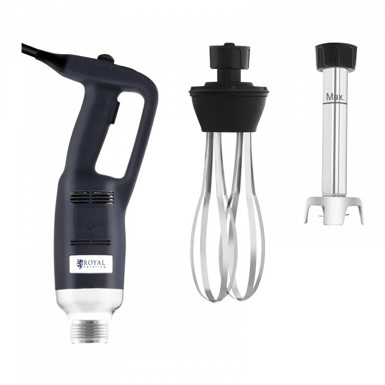
\includegraphics[scale=1]{../_res/mixer.png}
    \end{center}


    Därför yrkar vi
\begin{attsatser}
    \att stryka “Uppgradera utrustning i Edekvatas kök“ från beslutsuppföljningen
\end{attsatser}

\begin{signatures}{3}
    \signature{Filip Larsson}{Köksmästare 2018}
    \signature{Fredrik Berg}{Köksmästare 2018}
    \signature{Y Nhi Pham}{Preferensmästare 2018}
\end{signatures}

\end{document}
